\begin{problem}[26]
若硬度计的压头不是锥形而是球形, 可否分析硬度和强度在什么条件下成正比?
\end{problem}
% --------------------------------------------------------------------
\begin{solution}
\begin{minipage}[c]{0.7\linewidth}
设测试材料的杨氏模量为$E$, 屈服极限为$Y$, 塑性硬化指数为$n$, 泊松比为$\nu$. 给定材料和硬度计的压头半径为$R$. 那么载荷$F$和接触深度$h_c$应该由压入深度$h$唯一确定, 即有以下函数关系
\[
F = f_{F} (E, \nu; Y, n; h, R)
,\qquad
h_c = f_{h_c} (E, \nu; Y, n; h, R)
\]
\end{minipage}
\begin{minipage}[c]{0.3\linewidth}
\begin{center}
\usetikzlibrary{calc,intersections,through,backgrounds}
\usetikzlibrary{decorations.pathreplacing,decorations.pathmorphing,arrows}
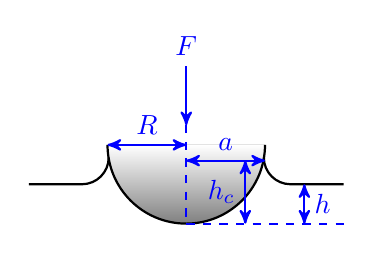
\begin{tikzpicture}
\fill[top color=white, bottom color=gray] (-1,0) arc(-180:0:1);
\draw[thick] (-1,0) arc(-180:0:1);
\draw[thick]  (-2,-0.5) -- (-1.325,-0.5) arc(-90:0:0.34);
\draw[thick]  (2,-0.5) -- (1.325,-0.5) arc(270:180:0.34);
\draw[thick,blue,dashed] (0,-1)--(2,-1) (0,0.25)--(0,-1);
\draw[thick,blue,<->,>=stealth'] (0,-0.2)--(1,-0.2) node[midway,above]{$a$};

\draw[thick,blue,<-,>=stealth'] (0,0.25)--(0,1) node[above]{$F$};
\draw[thick,blue,<->,>=stealth'] (0,0)--(-1,0) node[midway,above]{$R$};
\draw[thick,blue,<->,>=stealth'] (0.75,-1)--(0.75,-0.2) node[midway,left]{$h_c$};

\draw[thick,blue,<->,>=stealth'] (1.5,-1)--(1.5,-0.5) node[midway,right]{$h$};
\end{tikzpicture}
\end{center}
\end{minipage}
因为硬度$H$的定义为
\[
H = \frac{F}{\pi a^2}
, \quad\text{而}~
a = \sqrt{R^2 - (R-h_c)^2}
\]
所以$H$同样是上述自变量的函数, 即
\[
H = f_H(E, \nu; Y, n; h, R)
\]
选取$Y$和$R$作为基本量, 于是有
\[
%\frac{F}{Eh^2} = f_F \bigg(\nu; \frac{Y}{E}, n, \frac{R}{h}\bigg),\quad
%\frac{h_c}{h} = f_{h_c} \bigg(\nu; \frac{Y}{E}, n, \frac{R}{h}\bigg),\quad
\frac{H}{Y} = f_H\bigg(\frac{E}{Y},\nu, n, \frac{h}{R}\bigg)
\]
从上式可以看出$f_H$并不是常数, 只有当$E/Y\ll 1$且$h/R\ll 1$时, 才能近似的认为$H$与$Y$成正比. 但$h/R$并不满足$h/R\ll 1$, 且$h/R$随着$h$变化而变化, 因此, \textbf{不能断定硬度$H$和强度$Y$成正比}.
\end{solution}
